\documentclass{beamer}
%Information to be included in the title page:
\mode<presentation>

\usetheme{CambridgeUS}
\usecolortheme{beaver}

\usepackage{graphicx} % Required for inserting images
\usepackage{xcolor}


\title{Predstavitev prve domače naloge}
\author{Matija Debeljak}
\institute{Fakulteta za strojništvo}
\date{Oktober 2023}
\titlegraphic{
\includegraphics[width=2cm]{Slike/Logoulfs.jpg}}

\begin{document}


\frame{\titlepage}

\begin{frame}
\frametitle{Kazalo}
\section{ideja metode Monte Carlo}
\section{Kaj smo storili}
    \subsection{Funkcijske datoteke}
    \subsection{Programske datoteke}
    \subsection{Anonimne funkcije, vizualizacija}
\section{Rezultati}
\section{Zaključek}
\tableofcontents
\end{frame}

\begin{frame}
\frametitle{Ideja metode Monte Carlo}
\begin{center}
    

Metoda Monte Carlo deluje na osnovi naključnih števil.

\begin{figure}[h]
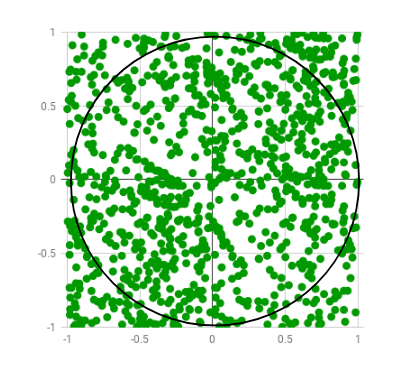
\includegraphics[scale=0.4]{Slike/MonteCarlo.png}
\caption{Naključno razporejena števila}
\end{figure}
\end{center}
\end{frame}

\begin{frame}
\frametitle{Ideja metode Monte Carlo}
Ustvarimo več naključnih števil, ki so od koordinatnega izhodišča oddaljena za največ 1.
        \begin{block}{Verjetnost, da so števila znotraj kvadrata 2x2}
        100\%
        \end{block}
        \begin{block}{Verjetnost, da so števila znotraj kroga r = 1}
        \dfrac{\pi}{4}
        \end{block}
        \begin{block}{Posledično lahko iz razmerja števil znotraj in zunaj kroga izračunamo približek števila $\pi$.}
        \Large
        \[ \pi = 4\cdot \frac{\text{število točk znotraj kroga}}{\text{število vseh točk}} \]
        
        \end{block}
        
\end{frame}



\begin{frame}{Kaj smo storili}
\begin{block}{1.1/ Funkcijske datoteke}
\begin{itemize}
\item Ustvarili smo funkcijo mcc\_pi, ki za vhod sprejme število naključnih točk.
\pause
\item Generira želejno število točk.
\pause
\item Izračuna ali so od izhodišča oddaljene za 1 ali manj (torej ležijo v krogu) ali več (ležijo izven kroga).
\end{itemize}    
\end{block}   
\end{frame}

\begin{frame}{Kaj smo storili}
\begin{block}{1.2/ Programske datoteke}
\begin{itemize}
\item Ustvarili smo programsko datoteko calc\_pi.
\pause
\item Datoteka kliče funkcijo mcc\_pi z naraščajočim številom naključnih števil.
\pause
\item Na grafu nariše vsak nov približek števila $\pi$ in njegovo oddaljenost od dejanskega števila $\pi$.
\end{itemize}
\end{block}
\end{frame}

\begin{frame}{Kaj smo storili}
\begin{block}{1.3 in 1.4/ Anonimne funkcije, vizualizacija}
\begin{itemize}
\item Napisali smo anonimno funkcijo  "krog", ki za vsak x izračuna dva y, ki ležita na krožnici r = 1.
\pause
\item Za vizualizacijo smo napisali program, ki s prej omenjeno anonimno funkcijo nariše krožnico.
\pause
\item nato pa nariše še točke, ki jih je generiral mcc\_pi, če ležijo znotraj kroga so zelene zvezdice, drugače so rdeče pike.
\end{itemize}
\end{block}
\end{frame}

\begin{frame}{Rezultati}

\begin{center}
    

\begin{figure}[h]
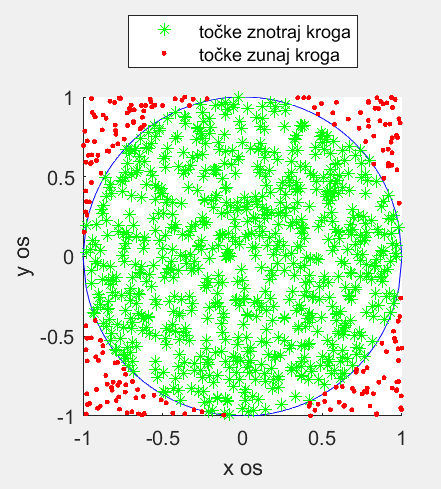
\includegraphics[scale=0.4]{Slike/tocke.png}
\caption{Graf naključno razporejenih točk}


\end{figure}
\end{center}

\end{frame}

\begin{frame}{Rezultati}

\begin{center}
    

\begin{figure}[h]

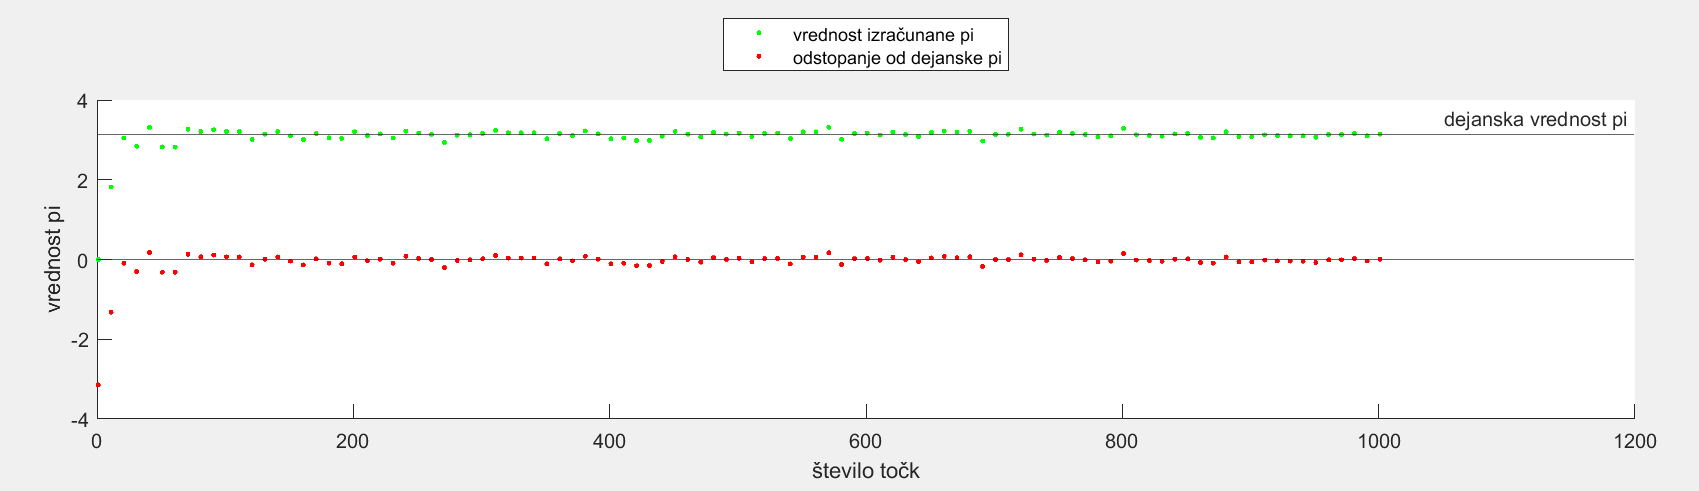
\includegraphics[scale=0.275]{Slike/graf pi.png}
\caption{Graf izračunane vrednosti pi}
\end{figure}
\end{center}

\end{frame}


\begin{frame}{Zaključek}
\begin{itemize}
\item Ustvarili smo program, ki generira željeno število naključnih števil.
\item Izračuna ali so števila znotraj krožnice r = 1 ali ne.
\item Iz generiranih točk izračuna približek števila $\pi$ in njegovo oddaljenost od dejanskega števila $\pi$.
\item Na koncu izriše graf vrednosti $\pi$ in napake za vsako iteracijo ter graf točk znotraj in zunaj kroga.

\end{itemize}
\end{frame}


\end{document}


